% This file provides the generic header that sets up the page formatting and
% common custom macro and environment definitions that can be used for an exercise
% or tutorial sheet in a university course.
%
% You can consult the `00-Header.sty` file for a full list of available macros.
%
% --------------------80-CHARACTER-SOURCE-LINE-WIDTH-GUIDE----------------------

% The documentclass is set to an a4 paper article using KOMA-script
\documentclass[paper=a4]{scrartcl}

\newcommand{\theauthor}{Hendrik Nolte}
\newcommand{\thecourse}{Tutorial for the Secure Workflow} % Course long name
\newcommand{\thecourseabbr}{} % e.g. PCHPC
\newcommand{\thetype}{Tutorial} % e.g. Exercise, Tutorial
\newcommand{\theorganization}{GWDG} % e.g. University Göttingen
\newcommand{\theinstitution}{AG-C} % e.g. Department of Computer Science
\newcommand{\theyear}{2022} %
\newcommand{\theexercisenumber}{1} % number of the exercise or tutorial
\newcommand{\thedate}{\today} % e.g. March 28, 2022
\newcommand{\theterm}{SoSe} % SoSe or WiSe 

\usepackage{00-Header} % Custom header and macros

\begin{document}
\date{\thedate}
\exercise{\theexercisenumber}

\parskip 8pt
\makesheetheader

\section*{Learning Objectives}
The learning objectives in the tutorial are to understand the individual steps of the \textit{Secure Workflow}. This should provide a deeper understanding of the individual measures taken to utilize secure compute capabilities on a shared HPC system. 

\textbf{Warning: Usually this Secure Workflow would be automated End-to-End on a Secure Client and the user would only call it in a parametrized fashion, e.g. through a GUI. In this tutorial we will manually go through the steps to get a detailed understanding.}

% \subsection*{Tools}

% What are the key points of this tutorial
%\begin{itemize}
%  \item 
%\end{itemize}

\tableofcontents

%\clearpage
\bigskip

% Tutorial overview
This Tutorial will guide you step-by-step through the \textit{Secure Workflow}. 
It was developed to provide secure processing capabilities for sensitive data, e.g. medical data.
In order to allow this, it needs to be ensured that \textbf{only} the legitimate user can access this data, explicitly excluding admins and, of course, attackers. 
The secure workflow is sketched in \cref{fig:secure_sbatch}. 

The fundamental idea is that from a secure client system, which could be a system located in a secured hospital infrastructure, all data is encrypted and uploaded to the (potentially unsecure) shared HPC system.
The keys \textbf{must not} be uploaded to the HPC system, since this would render the encryption useless, because an attacker would then get access to both, your data and your encryption key. 
Instead we are using a separate key management system, which is outside of the HPC system, and therefore shielded from an attacker on the HPC system.
Since the data needs to be decrypted during computations, dedicated and isolated compute nodes are required. 
These compute nodes are part of a dedicated, hidden partition \texttt{secure}. 


\begin{figure*}[!ht]
    \centerline{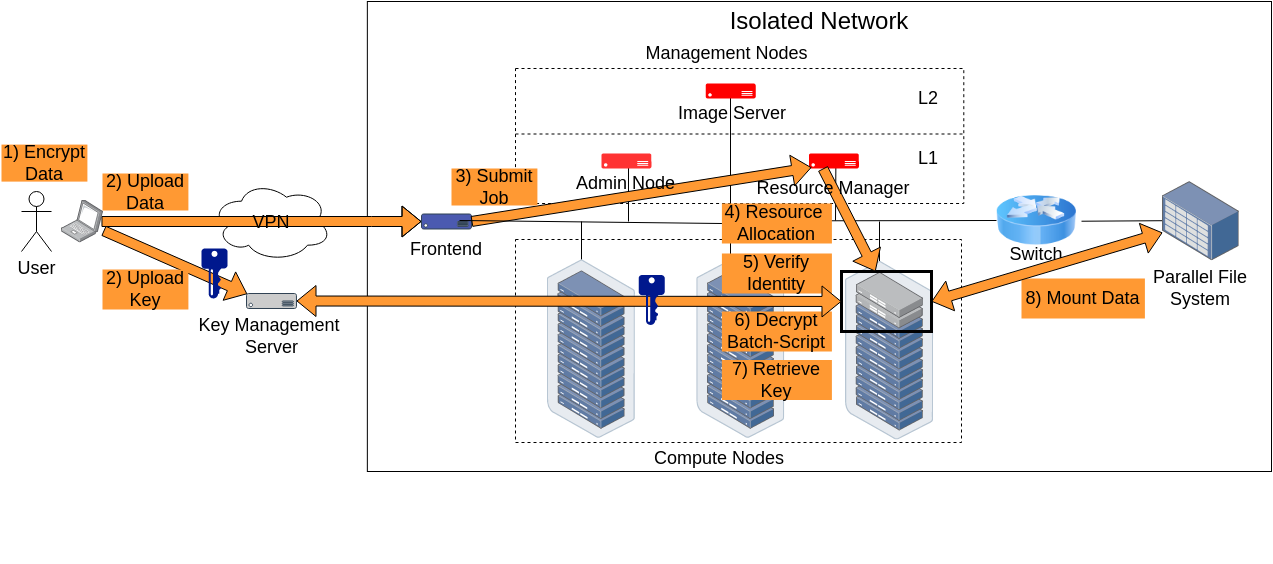
\includegraphics[width=0.8\textwidth]{secure_submission_neu.png}}
    \caption{A schematic sketch of the secure workflow on an HPC system, which is divided into 8 distinct steps. As shown, the sensitive data along with the container and the batch script are encrypted on the local machine of the user. Additionally, the batch script is also signed by the user. After encrypting, the components are safe to be uploaded into the shared file system of the HPC system. Although the batch script is signed and encrypted, it can be normally submitted in the third step. As usual, the resource manager will allocate the required resources and start the job in step 4). In the fifth step, the authenticity of the user request is verified and in the 6th step, the batch script is decrypted. Using the provided token for the key management system (KMS) the keys are retrieved in step 7 and used to decrypt the data and container on the isolated, secure node in step 8. }
    \label{fig:secure_sbatch}
\end{figure*}

\tutorial{The Secure Client}{10} % {name}{time in min}
As described in the synopsis, the secure client is always the beginning of a secure workflow. 
You should have gotten a \texttt{uid} and password. 
When you connect via \texttt{ssh}, you should be prompted for a password.

Please connect now to the secure client with:\\
\cmd{ssh <uid>@141.5.99.62} 
\\and enter the password when prompted. 

You should now be in your \texttt{\$HOME} and you can enter our \texttt{job\_template} directory with \cmd{cd job\_template}. 
Here you will find \texttt{src} directory containing a Singularity/Apptainer recipe. 
This can be used to build your container image to run \textit{BART}. 
The \texttt{data} directory contains your sample input data. 
In a real use case, this would be your medical data from a patient, which requires the highest protection. 

Now that you are on the secure client you will need access to the secure HPC server. 
You can access this via \texttt{ssh} again, but this time, instead of access via a password, you will be uploading your public ssh key onto LDAP.
\begin{figure*}[!ht]
    \centerline{
\includegraphics[width=0.65\textwidth]{gwdg1.png}}
    \caption{}
    \label{fig:screenshot1}
\end{figure*}
You can do that by signing into \href{https://www.gwdg.de} with your credentials. 
Once you're in, go to ``Mein Konto" via the drop-down on the top right. Under ``Andere", you should see an option ``Bearbeiten" for adding/removing SSH public keys. 
Copy your public key present at \texttt{/home/UID/.ssh/id\_rsa.pub} 

\begin{figure*}[!ht]
    \centerline{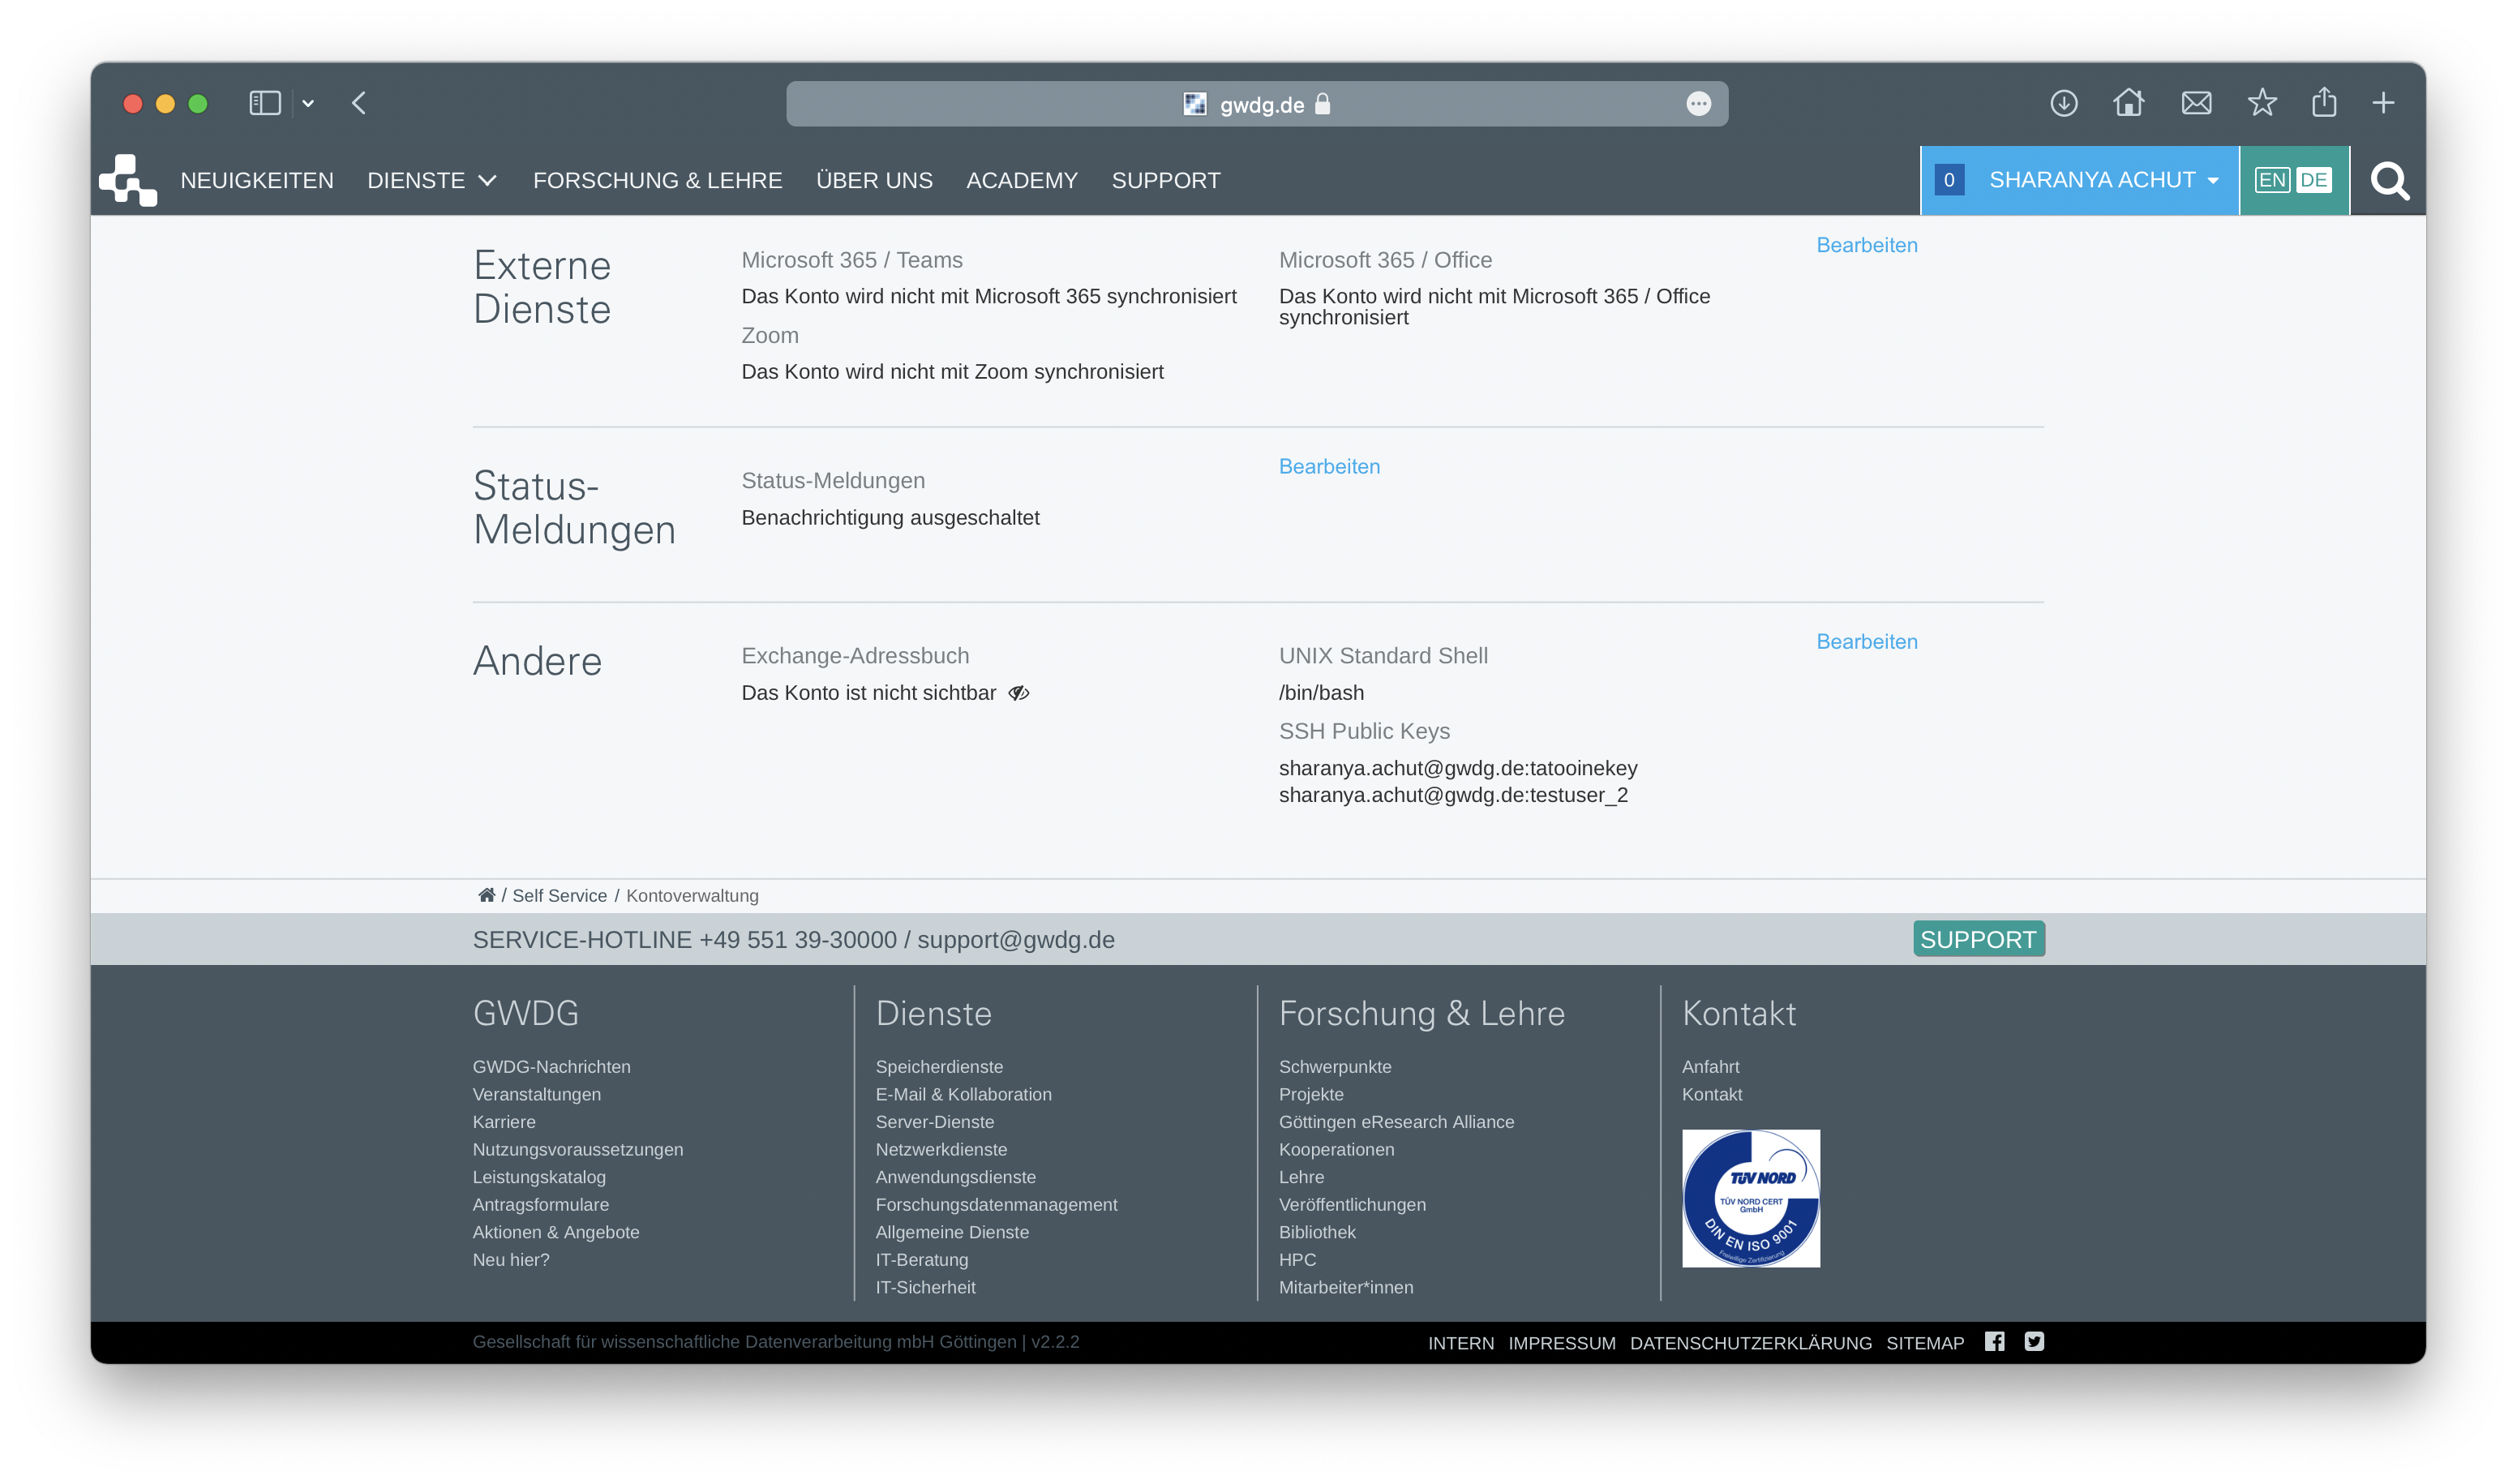
\includegraphics[width=0.65\textwidth]{gwdg2.png}}
    \caption{}
    \label{fig:screenshot2}
\end{figure*}

\begin{figure*}[!ht]
    \centerline{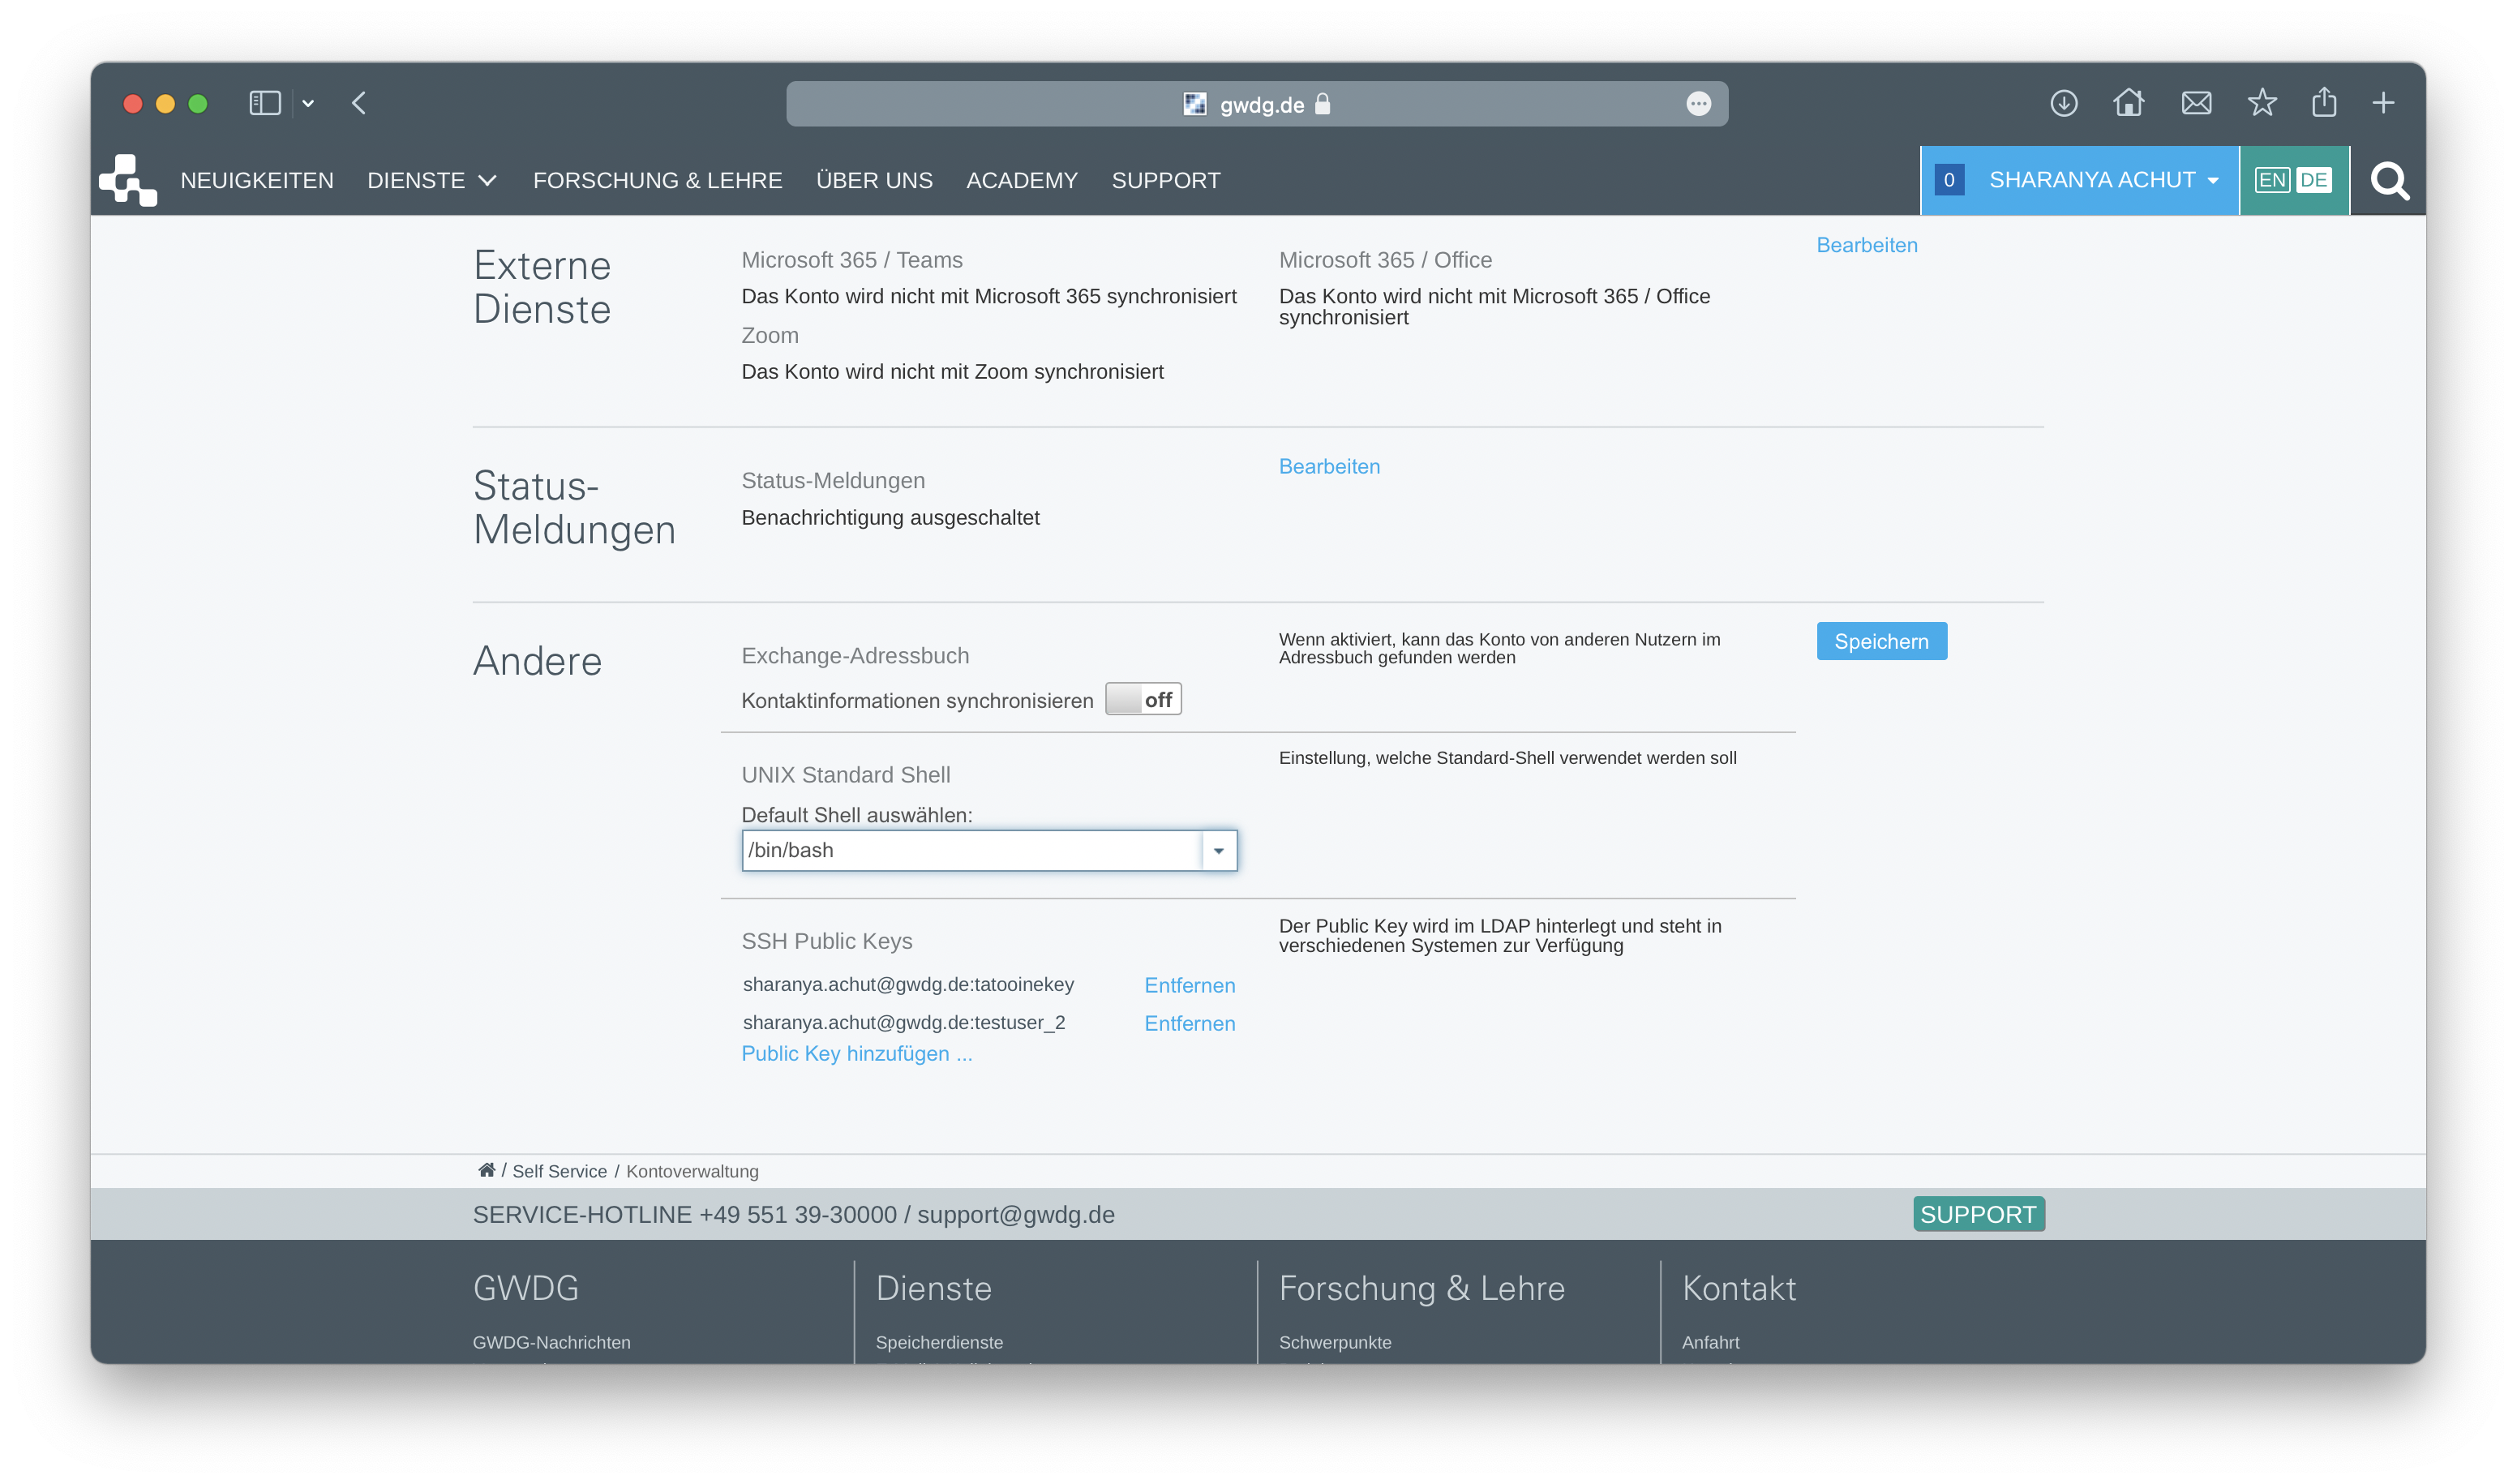
\includegraphics[width=0.65\textwidth]{gwdg3.png}}
    \caption{}
    \label{fig:screenshot3}
\end{figure*}
Once you upload your LDAP, you should be able to access the hpc cluster via ssh. 

\tutorial{Optional: End-to-End Automation}{5}
Once you login to the secure client via ssh, you can access \texttt{automatic.sh}, an end-to-end automation of the secure workflow that the rest of the tutorial walks you through. 
The script prepares your data container, encrypts uploads it, prepares yoxur batch script and executes it after encryption as well. Finally, the output is presented in a data container, mounted and ready to use. 
Before you run it, be sure to substitute the parametrized variables \texttt{$<$LUKScontainername$>$},\texttt{ $<$uid$>$}, \texttt{$<$hpc-uid$>$} and \texttt{$<$containername$>$} in \texttt{command.sh.template}. 

You can run \texttt{automatic.sh} with your \texttt{UID} of the secure client and \texttt{HPC-UID} as follows:\\
\texttt{./automatic.sh <uid> <hpc\_uid> <LUKScontainername>} \\

\tutorial{Encrypting the Data}{10}
The first step in the secure workflow is to encrypt your data. 
In this example, we will be using LUKS. 
To create a LUKS data container you can use a helper script located in \texttt{/opt/secure\_workflow/create\_data\_container.sh}. 
Executing it with the \texttt{-h} option provides you with information on how to execute it. 
It will show you, that you need to provide 3 parameters: 
\begin{itemize}
	\item The container name, which is an arbitrary name you can choose, e.g. myinputdata.
	\item The mount path on your local system, e.g. \texttt{/mnt/<uid>}, or \texttt{home/<client-uid>/<mymountpoint>}
	\item The size of your LUKS data container in MB to the basis of 10
\end{itemize}
So please go ahead on type: \\
\cmd{/opt/secure\_workflow/create\_data\_container.sh <containername> /mnt/<uid> 50} \\
Please notice, that you need to provide a minimal size of 50MB. \\
You can verify, that everything worked properly by doing a \cmd{ls /mnt/<uid>/<containername>}. 
If you see a fresh ext4 filesystem, indicated by the \texttt{lost+found} directory, it worked. 
You can now copy your input data into that container. 
Everything you write into that container is automatically encrypted. 
You can use for instance: \\
\cmd{cp data/* /mnt/<uid>/<containername>} \\
\cmd{ls /mnt/<uid>/<containername>}\\
You can now continue to umount the LUKS data container in order to be able to safely upload it to the HPC-system. 
We also have an wrapper script for that, you can just do: \\
\cmd{/opt/secure\_workflow/umount\_data\_container.sh <containername> /mnt/<uid>}
\\
If you look into your \texttt{\$pwd} you will see two new files:
\begin{itemize}
	\item \texttt{$<$containername$>$.img}
	\item \texttt{$<$containername$>$.key}
\end{itemize}
The *.img is your LUKS data container, which contains your encrypted data. This is secure to upload to the shared HPC system. 
The *.key file contains the key necessary to decrypt your data. This \textbf{must never} be uploaded to the HPC system, since an attacker would then have access to the encrypted data and also to the decryption key. 
Instead we will upload it to the dedicated Key Management System. 
But first we upload the LUKS data container:\\
\textbf{Please ensure beforehand that the directory exists}.
If it doesn't, you can do: \\
\cmd{ssh <hpc-uid>@gwdu101.gwdg.de 'mkdir /scratch/users/<hpc-uid>/secure'} \\
Then you can go ahead an upload your LUKS container into this directory: \\
\cmd{scp <containername>.img <hpc-uid>@transfer-scc.gwdg.de:/scratch/users/<hpc-uid>/secure} \\
\textbf{Please notice that the LUKS container has to be in exactly this folder.}

\tutorial{Building an Encrypted Singularity/Apptainer Container}{10}
In order to build a Singularity Container, you can use a helper script \texttt{buildEncryptedSingularity.sh}. 
Here, we use an RSA keypair to build an encrypted Singularity/Apptainer image with the recipe which you can find in \texttt{src/bart\_fft.def}. 
You can do the following: \\
\cmd{./buildEncryptedSingularity.sh} \\
\cmd{ls -lah bart\_fft\_enc.sif} \\
\textbf{Don't be confused if you see an Error message. One test might fail.} \\
You should see, that you successfully build your encrypted container. In order to be able to run it, you need your private key \texttt{rsa\_pri.key}. 
Since the container is encrypted you can securely upload it: \\
\cmd{ssh <hpc-uid>@gwdu101.gwdg.de 'mkdir /scratch/users/<hpc-uid>/home'} \\
\cmd{scp bart\_fft\_enc.sif <hpc-uid>@transfer-scc.gwdg.de:/scratch/users/<hpc-uid>/home}

\tutorial{Uploading Keys and Writing a Batch Script}{10}
Due to the encryption of our data and the encryption of the Singularity/Apptainer images, we have two keys, which we need to manage. 
These keys are uploaded into our Key Management System, i.e. Vault. 
In order to retrieve the keys later, we are receiving single-use and short-lived tokens from Vault. 
These tokens need to be included in the batch script, so that the keys can be retrieved on a secure node. 

The general \textit{command}, i.e. the bash-commands, is written in \texttt{command.sh.template}. 
Please open it in an editor, like vim, emacs or nano and substitute \textbf{only} the paramerized variables \texttt{$<$LUKScontainername$>$},\texttt{ $<$uid$>$}, \\\texttt{$<$hpc-uid$>$} and \texttt{$<$containername$>$}. 
(Note that \texttt{$<$LUKScontainername$>$} is the same as \texttt{$<$containername$>$}).

You can now execute \texttt{prepare\_scripts.sh} with: \\
\cmd{./prepare\_scripts.sh <local-uid> <LUKScontainername>} \\
This will upload your keys to Vault, and will insert the received tokens into a new file called \texttt{command.sh}. 
\texttt{command.sh} was automatically derived by \texttt{prepare\_scripts.sh} from your \texttt{command.sh.template}. 
\\
To summarize, your resulted \texttt{command.sh} is the bash-script,  that you want to execute on a secure node. 

\tutorial{Encrypting your Batch Script}{10}

Since it does contain the tokens to retrieve the keys from Vault, we should encrypt it as well. 
This can be done with \texttt{gpg}, for which you will import a public key on the secure client: \\
\cmd{gpg --import /tmp/agqkey}\\
There is a helper script,  \texttt{/opt/secure\_workflow/encrypt\_script.sh}, for encryption, which you can call as follows: \\
\cmd{/opt/secure\_workflow/encrypt\_script.sh command.sh agq001} \\
\textbf{If you get a warning, no problem, just go ahead and say yes} \\
This will encrypt your \texttt{command.sh} and will store it in \texttt{command.sh.asc}. 
\\
If you have a look at it, e.g. with \texttt{cat}, you will see that this is no bash script anymore, but an encrypted gpg message.
Since a valid bash script is required by Slurm, we need to provide one. 
For this passing in the encrypted gpg message to a \texttt{decrypt\_and\_execute} function, which we provide you on a secure node. 
The script that we want to submit to Slurm is called \texttt{run.sh}. 
Therefore, an encrypted script has to look exactly like this(of course, the actual message will be different): \\
\begin{lstlisting}[language=bash, caption=run.sh] 
#!/bin/bash

/usr/bin/decrypt_and_execute <<EOF
-----BEGIN PGP MESSAGE-----

hQIMA8ErHWKpRkmoAQ//daYFx4qwwc72XY2WavHv4RiEEArHqUXL1jVCATi/h8+c
hPkKL65KiAvExQgarvgJCRDhLt47F1HSUR3NT4pq1n1/Ql1Or2eSksUx8G6OoOia
KIDBceAyTe9joEb9PYMXHe4K2pJBt17GIWyBlX0c4ylzh/srSgbTNgxz7GnYJ8Qs
KwwjEpFaOy8f4Fuwir9ouKqNZnuQXLr/df6WDHAZYSQwvJcn26XhudvEEmQt6l3x
L/13fdWytwKoKvoqent+VuvXtYnq84Sk/rab+HwzuxfVuVgUEYe1yBQrOpyy62Bj
fQ1ZGWNigjjfQXY+pxHhDuk08CIMWUBfVpZ0To3D/ppnJiJvIjhRu9zvM3vZYXLT
7Nb00ZPQDiaDoap1k7msPh49QmdPk9VNgEPLx/fmMW9NJYXLGOcMv9JDTX7zguoT
eJEbmyZoo7mL5XPycPCPoYZrZcVvYjCgya6uWZp6tOYCuwIQzf7qM+puqlS3WnEg
rZvgiD1Ju80B6pB5cHPDhuB8+x7M9vSSzFF8LwuCj+/YfYPQkymoGdSaDIYdB2Fz
caqAhlWd/Z8MG9l+8JZbUpuLkg57jTWqI7qSSmHPJZu7rpAe5p8nTHRMhZ8IdkiO
uk06zSoQX42PaUPZMQZfAJE/NNxC5uAJ8xkBMzXF/ymRaboyETuxalmw3vyX1J7S
wTcBi66cufsqH45W4srKptKNKQpAf5M9JfRmXfHsQBzxwh8mWJ9gFmsrsaC6tTK1
KLeLapzVafnIk8/nvjxBmKRSc35GosWTi/AFKk8gj4FuSYtiUbFk8qggcXEVf18v
rE0VHAUIkFcdJ78y0slEx4ARu3vkCO+8+ublmyieF6lzRIh6ETdQAVpbrSfEVUnb
F/MJHeIrbED4tFp7VpwRwO459b4E77sMSAOI1xbWXWcpcJNLrkcR3K5fCsYrxnYd
r22ew3T3gAGX2SzaAYgaWGLHeLODvQMIgwBT47Fe32OjbngXMD1AAz5YqjKkLxMN
onErf2US19R5RXDAH0pAMT0Q+u4XVGCx6rbE/4ySV44tbV+6qyy68/dBzP0o+Zvz
Jnp5nmlpu8h3u6MTmOKypwOQUT4uxfe5J04NtIHT2GzYm1yINcOBBJqb3+MI2SNJ
S5us8whI/Srwz1J0PWCpx3XR/IoVe+rrw560ik2NaGDd0rk9IhHLbd+NAXm2aC9P
9BJbdyqiU7TxyZ7+2WKycTYULz67qo/B+On2YjWwh24yYWKbFYZPjCq1vhyfCNPa
bO6EDMdhYcTkFFOJABd/Lx4v8dfO35hFo11EmawYG7bIvF4qEFDRPLROCrbII89h
/O2S+G/v2huFNK1zO95WKXkOPqb1GiNlvg==
=Vq+R
-----END PGP MESSAGE-----
EOF
\end{lstlisting}
\textbf{Please notice the peculiar looking two EOF's!} \\
\textbf{Of course, you need to insert your own gpg message}

\tutorial{Signing your Batch Script and Securely Submitting Your Job}{10}
Since the integrity of the secure nodes depends on the restricted access, to prevent an attacker from accessing the node and tampering with it, we need to sign our batch script, to authenticate ourselves on the secured node. 
For this, a public-private key pair was generated, where the public key is imported on the secure node and the private key is only stored on the secure client. 
With this private key, we can do a detached signature. 
\\
\textbf{Please realize: The integrity of this entire workflow depends on the security of this private key with which we authenticate ourselves.}
\\
We import the private key, and perform the detached signature with: \\
\cmd{gpg --import /tmp/user\_priv}\\ 
\cmd{gpg --detach-sign --local-user user\_key -o run.sh.sig run.sh} \\
\textbf{You will be prompted for a passphrase. It is: test} \\
This will read in your \texttt{run.sh} create an additional file called \texttt{run.sh.sig}. 
You will need both files to submit your job on the HPC-System.
Please upload both of them into the same folder: \\
\cmd{scp run.sh run.sh.sig <hpc-uid>@gwdu101.gwdg.de:/scratch/users/<hpc-uid>/home/}
\\
You can now submit your job with: \\
\cmd{ssh <hpc-uid>@gwdu101.gwdg.de 'cd /scratch/users/<hpc-uid>/home ; /opt/slurm/bin/sbatch -p secure --exclusive run.sh'}
\\
After a few seconds, your job will be finished.
\\
The result should be stored in the same LUKS data container. 
You can fetch it again via \texttt{scp} as follows: \\
\cmd{scp <hpc-uid>@transfer-scc.gwdg.de:/scratch/users/<hpc-uid>/secure/<containername>.img .}
\\
You can then mount the container (provided that your key lies in the same directory) with: \\
\cmd{/opt/secure\_workflow/mount\_container.sh <containername>} \\
and then you can: \\
\cmd{ls -lah /mnt/<uid>/<containername>/}\\
You should see two new files: \texttt{output\_fft.cfl} and  \texttt{output\_fft.hdr}

\tutorial{Optional: Quick Summary if You Need to Repeat}{10}
This is a quick summary if you encountered at some point an Error.\\
Create an LUKS data container:\\
\cmd{/opt/secure\_workflow/create\_data\_container.sh <containername> /mnt/<uid> 50} \\
Copy your data into it:\\
\cmd{cp data/* /mnt/<uid>/<containername>} \\
\cmd{ls /mnt/<uid>/<containername>}\\
And umount it:
\cmd{/opt/secure\_workflow/umount\_data\_container.sh <containername> /mnt/<uid>}\\
Make all the necessary changes in \texttt{prepare\_script.sh} and \texttt{command.sh.template} and then execute:\\
\cmd{./prepare\_scripts.sh}\\
Encrypt your resulting \texttt{command.sh} which contains your KMS tokens:\\
\cmd{/opt/secure\_workflow/encrypt\_script.sh command.sh agq001} \\
Make a detached signature to authenticate on the secured node: \\
\cmd{gpg --detach-sign --local-user user\_key -o run.sh.sig run.sh} \\
Upload and submit your Job:
\cmd{scp run.sh run.sh.sig <hpc-uid>@gwdu101.gwdg.de:/scratch/users/<hpc-uid>/home/}
\\
\cmd{ssh <hpc-uid>@gwdu101.gwdg.de 'cd /scratch/users/<hpc-uid>/home ; /opt/slurm/bin/sbatch -p secure --exclusive run.sh'}\\
You can also check your Slurm output file in \texttt{/scratch/users/<hpc-uid>/home} to see if it worked.

\tutorial{Optional: Getting to Know the Job}{10} % {name}{time in min}
The command that we actually want to execute is \\
\cmd{./bart\_fft.sif ../data/shepp\_logan} \\
which will do \texttt{bart fft -u -i}, i.e. an inverse Fourier Trafo.
You can look at the images using \texttt{bart toimg}.
At first, you have an frequency/k-space image:

\begin{figure*}[!ht]
    \centerline{
\includegraphics[width=0.3\textwidth]{kraum.png}}
    \caption{K-Space image of Shepp-Logan}
    \label{fig:kraum}
\end{figure*}

\begin{figure*}[!ht]
    \centerline{
\includegraphics[width=0.3\textwidth]{realspace.png}}
    \caption{K-Space image of Shepp-Logan}
    \label{fig:realspace}
\end{figure*}

\end{document}